\chapter{Měření v rovnovážném stavu}\label{navesti:rovnovaznaMereni}
Pro ověření modelu výpočtu přísunu radonu z měření v rovnovážném stavu (viz kapitola~\ref{navesti:model}) mi byla poskytnuta data naměřená pro SÚRO (Státní ústav radiační ochrany, v. v. i.) v Bulharsku. Měření probíhala v osmi objektech v lednu a únoru 2019 a pomocí techniky indikačních plynů byly změřeny objemové objemové průtoky vzduchu mezi stanovenými kompartmenty všech objektů. OAR ve všech objektech byly změřeny integrálními detektory radonu (konkrétně elektretovými dozimetry, viz kapitola~\ref{navesti:radon}), avšak bohužel pouze u objektů č. 1, 2, 3, 4 a 8 byly OAR změřeny ve všech zónách, což je předpoklad pro použití modelu výpočtu přísunů radonu do jednotlivých zón.

V tab.~\ref{tab:rovMer_objekty} jsou adresy a počty podlaží všech použitelných objektů spolu s obdobím, kdy byly v daném objektu měřeny průtoky vzduchu mezi zónami a OAR v jednotlivých zónách. Jako zóny byly v každém objektu brány podlaží, tj. počet pater daného objektu určuje počet kompartmentů, na něž je rozdělen.
\begin{table}[ht]
	\centering
	\caption{Adresy a počty podlaží každého použitelného objektu. $T$ je doba měření absorpce indikačních plynů v TD detektorech a zároveň je to i doba měření OAR v jednotlivých zónách. Čtvrtý sloupec udává počátek těchto měření.}
	\label{tab:rovMer_objekty}
\begin{tabular}{llllll}
	\toprule 
&Adresa&Počet podlaží&Počátek měření&$T$ [dny]&Použitelné\\
	\midrule 
1	& Sofia, Kalach 20 & 3 & 31. 1. 2019 10:30 & 29,0 & ANO\\ 
2	& 42\degree41'00.7''N 26\degree20'00.5''E &1  &29. 1. 2019 10:00 &28,1 &ANO \\ 
3	& 42\degree42'01.0"N 25\degree52'21.6"E & 2 &28. 1. 2019 16:00  &28,8 & ANO\\ 
4	& Sofia, Yaroslav Hashek 36 & 2 & 31. 1. 2019 13:00 & 26,0& ANO\\ 
5	&  &  &  & & NE\\ 
6	&  &  &  & & NE\\ 
7	&  &  &  & & NE\\ 
8	& 42\degree08'14.6"N 24\degree44'26.5"E &3  & 29. 1. 2019 15:30 & 28,9& ANO\\ 
	\bottomrule
\end{tabular} 
\end{table}

V následujících podkapitolách jsou uvedeny naměřené veličiny (průtoky vzduchu, OAR, objemy) a vypočítané přísuny radonu do všech zón. U uváděných nejistot je uvažován faktor pokrytí $k=1$, tj. nejistoty jsou rovny směrodatným odchylkám. Podlaží jsou udávána jako čísla, viz tab.~\ref{tab:rovMer_podlazi}. Koncentrace radonu vnějšího prostředí $OAR_{out}$ nebyla ani v jednom případě změřena, a proto byly přísuny radonu vypočteny pro několik jejích typických hodnot: $0, 5, 10, 20, 30\ \si{Bq/m^3}$. Nejistota všech objemů byla odhadnuta na 20~\% nominální hodnoty.
\begin{table}[ht]
	\centering
	\caption{Význam značení podlaží v následujících podkapitolách.}
	\label{tab:rovMer_podlazi}
	\begin{tabular}{ll}
		\toprule
		0&sklep\\
		1&přízemí\\
		2&první patro\\
		\bottomrule
	\end{tabular}
\end{table}

\section{Objekt č. 1}
První tabulka v tomto oddíle obsahuje naměřené OAR a objemy všech zón (tj. podlaží). Pokud bylo naměřeno více hodnot OAR v nějaké zóně, pak byl z nich byl udělán průměr. Druhá tabulka průtoky vzduchu mezi zónami, exfiltrace zón a dopočítané infiltrace zón. Ve třetí tabulce jsou vypočítané přísuny radonu. 

Podkapitoly ostatních objektů mají stejnou strukturu.
\begin{table}[H]
	\centering
	\caption{Průměrné koncentrace radonu v daném podlaží a objemy všech místností v daném podlaží.}
	\begin{tabular}{lll}
\toprule
podlazi & $OAR$ [\si{Bq/m^3}] & $V$ [\si{m^3}] \\
\midrule
0 &           1094+/-55 &         40+/-8 \\
1 &            562+/-20 &        84+/-10 \\
2 &              51+/-2 &        97+/-15 \\
\bottomrule
\end{tabular}

\end{table}
\begin{table}[H]
	\centering
    \caption{Objemové průtoky vzduchu mezi zónami v \si{m^3/hod} a celková výměna vzduchu objektu $n$ v \si{hod^{-1}}. Přiřazení zón podlažím objektu je vzestupné, tj. první zóna je sklep, druhá zóna přízemí a třetí zóna je první patro.}
	\begin{tabular}{lr}
\midrule
$k_{12}$   &  $1,32 \pm0,37 $\\
$k_{13}$   &  $0,03 \pm0,03 $\\
$k_{21}$   &  $2,50 \pm0,75 $\\
$k_{23}$   &  $0,47 \pm0,16 $\\
$k_{31}$   &  $0,14 \pm0,12 $\\
$k_{32}$   &  $1,26 \pm0,37 $\\
&\\                       
$k_{1_E}$   & $45,26\pm 7,75$ \\
$k_{2_E}$   & $23,02\pm 4,17$ \\
$k_{3_E}$   & $16,24\pm 2,86$ \\
$k_{1_I}$   & $43,97\pm 7,80$ \\
$k_{2_I}$   & $23,40\pm 4,27$ \\
$k_{3_I}$   & $17,14\pm 2,89$ \\
\midrule
$n$         & $0,38 \pm 0,05$ \\
\bottomrule
\end{tabular}

\end{table}
\begin{table}[ht]
	\centering
	\caption{Výsledné přísuny radonu pro několik případů koncentrací radonu ve vnějším prostředí. $Q_i$ značí přísun radonu do $i$-tého podlaží.}
    \label{tab:rovMer_Q_1}
	\begin{tabular}{llll}
\toprule
$OAR_{out}$ [\si{Bq/m^3}] & $Q_0$ $\left[\si{\frac{Bq}{m^3\cdot hod}}\right]$ & $Q_1$ $\left[\si{\frac{Bq}{m^3\cdot hod}}\right]$ & $Q_2$ $\left[\si{\frac{Bq}{m^3\cdot hod}}\right]$ \\
\midrule
0  &                                        1256+/-335 &                                          160+/-35 &                                             7+/-2 \\
5  &                                        1250+/-334 &                                          159+/-34 &                                             6+/-2 \\
10 &                                        1245+/-332 &                                          157+/-34 &                                             5+/-2 \\
20 &                                        1234+/-329 &                                          154+/-33 &                                             3+/-1 \\
30 &                                        1223+/-326 &                                          152+/-33 &                                             1+/-1 \\
\bottomrule
\end{tabular}

\end{table}

\section{Objekt č. 2}
\begin{table}[H]
	\centering
	\caption{Průměrné koncentrace radonu v daném podlaží a objemy všech místností v daném podlaží.}
	\begin{tabular}{lll}
\toprule
podlazi & $OAR$ [\si{Bq/m^3}] & $V$ [\si{m^3}] \\
\midrule
1 &           1357+/-41 &        91+/-11 \\
\bottomrule
\end{tabular}

\end{table}
\begin{table}[H]
	\centering
    \caption{Exfiltrace a infiltrace jediné zóny objektu v \si{m^3/hod}, jedná se tedy vlastně o exfiltraci a infiltraci celého objektu. $n$ je výměna vzduchu objektu v \si{hod^{-1}}.}
	\begin{tabular}{lll}
\toprule
{} &       1 & vnější prostředí \\
\midrule
1                &       0 &           45$\pm$9 \\
vnější prostředí &  45$\pm$9 &                0 \\
\bottomrule
\end{tabular}

\end{table}
\begin{table}[H]
	\centering
	\caption{Výsledné přísuny radonu pro několik případů koncentrací radonu ve vnějším prostředí. $Q_i$ značí přísun radonu do $i$-tého podlaží.}
    \label{tab:rovMer_Q_2}
	\begin{tabular}{ll}
\toprule
$OAR_{out}$ [\si{Bq/m^3}] & $Q_1$ $\left[\si{\frac{Bq}{m^3\cdot hod}}\right]$ \\
\midrule
0  &                                         683$\pm$157 \\
5  &                                         681$\pm$157 \\
10 &                                         678$\pm$156 \\
20 &                                         673$\pm$155 \\
30 &                                         668$\pm$154 \\
\bottomrule
\end{tabular}

\end{table}

\section{Objekt č. 3}
\begin{table}[H]
	\centering
	\caption{Průměrné koncentrace radonu v daném podlaží a objemy všech místností v daném podlaží.}
	\begin{tabular}{lll}
\toprule
podlazi & $OAR$ [\si{Bq/m^3}] & $V$ [\si{m^3}] \\
\midrule
1 &          3042$\pm$108 &         77$\pm$8 \\
2 &             211$\pm$7 &         65$\pm$8 \\
\bottomrule
\end{tabular}

\end{table}
\begin{table}[H]
	\centering
    \caption{Objemové průtoky vzduchu mezi zónami v \si{m^3/hod} a celková výměna vzduchu objektu $n$ v \si{hod^{-1}}. Přiřazení zón podlažím objektu je vzestupné: první zóna je přízemí a druhá zóna je první patro.}
	\begin{tabular}{llll}
\toprule
{} &          1 &          2 & vnější prostředí \\
\midrule
1                &          0 &  3.2+/-0.9 &           50+/-9 \\
2                &  1.7+/-0.5 &          0 &          56+/-10 \\
vnější prostředí &     51+/-9 &    54+/-10 &                0 \\
\bottomrule
\end{tabular}

\end{table}
\begin{table}[H]
	\centering
	\caption{Výsledné přísuny radonu pro několik případů koncentrací radonu ve vnějším prostředí. $Q_i$ značí přísun radonu do $i$-tého podlaží.}
    \label{tab:rovMer_Q_3}
	\begin{tabular}{lll}
\toprule
$OAR_{out}$ [\si{Bq/m^3}] & $Q_1$ $\left[\si{\frac{Bq}{m^3\cdot hod}}\right]$ & $Q_2$ $\left[\si{\frac{Bq}{m^3\cdot hod}}\right]$ \\
\midrule
0  &                                        2120$\pm$418 &                                           37$\pm$55 \\
5  &                                        2117$\pm$417 &                                           32$\pm$55 \\
10 &                                        2113$\pm$416 &                                           28$\pm$54 \\
20 &                                        2107$\pm$415 &                                           20$\pm$53 \\
30 &                                        2100$\pm$414 &                                           11$\pm$52 \\
\bottomrule
\end{tabular}

\end{table}

\section{Objekt č. 4}
\begin{table}[H]
	\centering
	\caption{Průměrné koncentrace radonu v daném podlaží a objemy všech místností v daném podlaží.}
	\begin{tabular}{lll}
\toprule
podlazi & $OAR$ [\si{Bq/m^3}] & $V$ [\si{m^3}] \\
\midrule
1 &            433$\pm$22 &       119$\pm$20 \\
2 &             208$\pm$7 &       102$\pm$14 \\
\bottomrule
\end{tabular}

\end{table}
\begin{table}[H]
	\centering
    \caption{Objemové průtoky vzduchu mezi zónami v \si{m^3/hod} a celková výměna vzduchu objektu $n$ v \si{hod^{-1}}. Přiřazení zón podlažím objektu je vzestupné: první zóna je přízemí a druhá zóna první patro.}
	\begin{tabular}{l
        >{\collectcell\num}r<{\endcollectcell}
        @{${}\pm{}$}
        >{\collectcell\num}r<{\endcollectcell}
    }
\toprule
$k_{12}$                 &        \multicolumn{2}{r}{$15\pm\ \, 4$} \\
$k_{21}$                 &        \multicolumn{2}{r}{$15\pm\ \, 4$} \\
&\multicolumn{2}{r}{}\\                                        
$k_{1_E}$                 &       \multicolumn{2}{r}{$27\pm\ \, 7$} \\
$k_{2_E}$                 &       \multicolumn{2}{r}{$44\pm\ \, 9$} \\
$k_{1_I}$                 &       \multicolumn{2}{r}{$28\pm\ \, 9$} \\
$k_{2_I}$                 &       \multicolumn{2}{r}{$43\pm11$} \\
\midrule
$n$                   &            0,32 &      0,04 \\
\bottomrule
\end{tabular}

\end{table}
\begin{table}[H]
	\centering
	\caption{Výsledné přísuny radonu pro několik případů koncentrací radonu ve vnějším prostředí. $Q_i$ značí přísun radonu do $i$-tého podlaží.}
    \label{tab:rovMer_Q_4}
	\begin{tabular}{lll}
\toprule
$OAR_{out}$ [\si{Bq/m^3}] & $Q_1$ $\left[\si{\frac{Bq}{m^3\cdot hod}}\right]$ & $Q_2$ $\left[\si{\frac{Bq}{m^3\cdot hod}}\right]$ \\
\midrule
0  &                                          131$\pm$38 &                                           55$\pm$29 \\
5  &                                          130$\pm$37 &                                           53$\pm$29 \\
10 &                                          129$\pm$37 &                                           51$\pm$28 \\
20 &                                          126$\pm$36 &                                           46$\pm$27 \\
30 &                                          124$\pm$35 &                                           42$\pm$26 \\
\bottomrule
\end{tabular}

\end{table}

\section{Objekt č. 8}
\begin{table}[H]
	\centering
	\caption{Průměrné koncentrace radonu v daném podlaží a objemy všech místností v daném podlaží.}
    \label{tab:rovMer_namereno_8}
	\begin{tabular}{lll}
\toprule
podlazi & $OAR$ [\si{Bq/m^3}] & $V$ [\si{m^3}] \\
\midrule
0 &              33+/-2 &        66+/-13 \\
1 &              61+/-3 &       105+/-11 \\
2 &              79+/-2 &       153+/-15 \\
\bottomrule
\end{tabular}

\end{table}
\begin{table}[H]
	\centering
    \caption{Objemové průtoky vzduchu mezi zónami v \si{m^3/hod} a celková výměna vzduchu objektu $n$ v \si{hod^{-1}}. Přiřazení zón podlažím objektu je vzestupné: první zóna je sklep, druhá zóna přízemí a třetí zóna je první patro.}
    \label{tab:rovMer_prutoky_8}
	\begin{tabular}{lrr}
\toprule
{} &  hodnota $\left[\si{m^3/hod}\right]$ &  $\sigma$ \\
\midrule
k12                 &                                 9,29 &      3,26 \\
k13                 &                                 6,81 &      3,88 \\
k14                 &                                90,66 &     17,27 \\
k21                 &                                41,48 &     12,49 \\
k23                 &                                30,11 &     13,92 \\
k24                 &                               134,74 &     32,68 \\
k31                 &                                54,32 &     22,01 \\
k32                 &                                58,73 &     25,38 \\
k34                 &                               533,82 &    128,35 \\
k41                 &                                10,96 &     31,05 \\
k42                 &                               138,30 &     45,53 \\
k43                 &                               609,95 &    133,46 \\
n                   &                                 2,34 &      0,40 \\
n $[\si{hod^{-1}}]$ &                                 2,35 &      0,44 \\
\bottomrule
\end{tabular}

\end{table}
\begin{table}[H]
	\centering
	\caption{Výsledné přísuny radonu pro několik případů koncentrací radonu ve vnějším prostředí. $Q_i$ značí přísun radonu do $i$-tého podlaží.}
    \label{tab:rovMer_Q_8}
	\begin{tabular}{llll}
\toprule
$OAR_{out}$ [\si{Bq/m^3}] & $Q_0$ $\left[\si{\frac{Bq}{m^3\cdot hod}}\right]$ & $Q_1$ $\left[\si{\frac{Bq}{m^3\cdot hod}}\right]$ & $Q_2$ $\left[\si{\frac{Bq}{m^3\cdot hod}}\right]$ \\
\midrule
0  &                                          -50$\pm$32 &                                           73$\pm$31 &                                          322$\pm$76 \\
5  &                                          -50$\pm$30 &                                           67$\pm$29 &                                          302$\pm$71 \\
10 &                                          -51$\pm$28 &                                           60$\pm$26 &                                          282$\pm$67 \\
20 &                                          -53$\pm$24 &                                           47$\pm$22 &                                          242$\pm$57 \\
30 &                                          -55$\pm$21 &                                           34$\pm$18 &                                          202$\pm$48 \\
\bottomrule
\end{tabular}

\end{table}

\section{Diskuze}
V tabulkách~\ref{tab:rovMer_Q_1}, \ref{tab:rovMer_Q_2}, \ref{tab:rovMer_Q_3}, \ref{tab:rovMer_Q_4} a \ref{tab:rovMer_Q_8} jsou vypočítané přísuny radonů pro objekty č. 1, 2, 3, 4 a 8. Je vidět, že všechny kromě osmého objektu se řídí tím, co bylo uvedeno v podkapitole~\ref{navesti:model_interpretace_Q}, tj. čím dále je zóna od geologického podloží, tím je přísun radonu do ní menší. 

U osmého objektu je vývoj velikostí přísunů radonu opačný, než bychom předpokládali. Stačí se ovšem podívat na tabulku naměřených OAR v jednotlivých zónách~\ref{tab:rovMer_namereno_8} a vidíme, proč tomu tak je: OAR je nejvyšší v prvním patře, pak v přízemí a ve sklepě je nejmenší. Toto je velmi nezvyklé a pokud se nejedná o chybu měření (vzhledem k údajům z tabulky~\ref{tab:rovMer_8diskuze} nepravděpodobné, viz dále), pak je to důsledek nějaké anomálie. Pro větší názornost jsou v tab.~\ref{tab:rovMer_8diskuze} zobrazeny hodnoty OAR naměřené v místnostech osmého objektu; OAR uvedené v tab.~\ref{tab:rovMer_namereno_8} jsou pak průměrem přes danou zónu/podlaží. Vidíme, že vyšší koncentrace než ve sklepu byly naměřeny ve všech místnostech v přízemí i v prvním patře a že v ložnice v prvním
patře byla naměřena dvojnásobná koncentrace radonu než v ostatních místnostech. S přihlédnutím ke schématu domu (obr.~\ref{fig:rovMer_8schema}) si lze domýšlet, že ložnice v prvním patře je v kontaktu s podložím a na rozdíl od sklepa nemá tak dobrou radonovou izolaci. Odtud by se radon mohl šířit do dalších částí domu. Fotky objektu, které by nám tuto hypotézu potvrdily, bohužel nejsou k dispozici.

Za zmínku také stojí záporně vycházející přísun radonu do sklepa. Lze to přisoudit nepřesnostem vzniklých při měření. Avšak uváděná nejistota je rovna směrodatné odchylce $\sigma$ a tudíž $Q_0$ je v rámci rozšířené nejistoty nezáporný.
%Je možné, že stavební materiál v prvním patře obsahuje velký obsah uranu, nebo že v prvním patře je nějaký jiný zdroj radonu. Vzhledem k vysoké koncentraci radonu lze předpokládat hlavní umístění tohoto zdroje v ložnici. 
%Je možné uvažovat, že vyšší OAR v přízemí a v prvním patře je dána velkou koncentrací radonu ve vnějším prostředí, jelikož tyto podlaží mají o řád větší inhalaci než sklep (viz tab.~\ref{tab:rovMer_prutoky_8}). První patro má největší inhalaci ze všech podlažích, a proto má největší přísun radonu. To, že ložnice v prvním patře má největší naměřenou koncentraci radonu, by šlo přisoudit tomu, že se v ložnici nejvíc větrá. Této úvaze dále přihrávají n, že průtoky ze sklepa do ostatních zón jsou malé, což znamená, že podlaží není hlavním zdrojem radonu v tomto objektu. 
\shorthandoff{-}
\begin{table}[ht]
	\centering
    \caption{Přebraná tabulka z~\cite{rovMer_8Rn} obsahující naměřené koncentrace radonu v některých místnostech objektu č. 8.}
	\label{tab:rovMer_8diskuze}
	\begin{tabular}{llp{2cm}p{3cm}}
		\toprule
		\multirow{2}{*}{Location in dwelling} & \multirow{2}{*}{Period from\ldots to}  & \multicolumn{2}{l}{Results of measurements [\si{Bq/m^3}]} \\
		\cline{3-4}
		&   & Radon concentration   & Combined standard uncertainty (1$\sigma$)   \\
		\midrule
		Dining room, floor 2    & 29.01.2019 to 27.02.2019 & 66 & 3  \\
		Living room,   floor 2 & 29.01.2019   to 27.02.2019 & 51  & 3 \\
		Bedroom 2, floor 2& 29.01.2019   to 27.02.2019 & 120  & 6   \\
		Living room, floor 1 &29.01.2019   to 27.02.2019 & 61 & 3  \\
		Basement   & 29.01.2019   to 27.02.2019 & 33  & 2 \\
		\bottomrule
	\end{tabular}
\end{table}
\shorthandon{-}
\begin{figure}[ht]
    \centering
    \begin{subfigure}{.49\textwidth}
        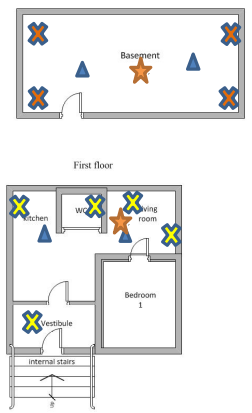
\includegraphics[width=.95\textwidth]{rovMer_8schema.png}
        %\caption{}
    \end{subfigure}
    \begin{subfigure}{.49\textwidth}
        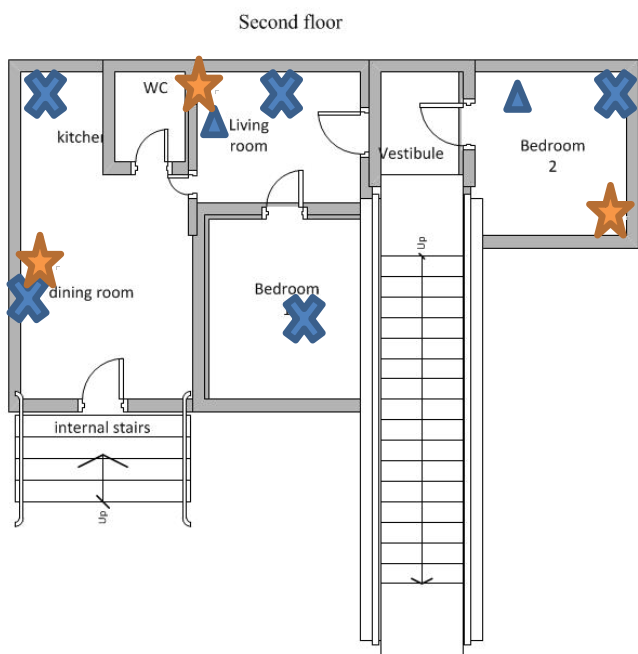
\includegraphics[width=.95\textwidth]{rovMer_8schema_2.png}
        %\caption{}
    \end{subfigure}
    \caption{Schéma objektu č. 8. Křížky značí vyvíječe, trojúhelníky TD detektory a hvězdičky elektretové dozimetry. \cite{rovMer_8Rn}}
    \label{fig:rovMer_8schema}
\end{figure}

Dále lze vypozorovat, že u všech objektů se přísuny radonu do všech zón zmenšují se zvyšující se koncentrací radonu ve vnějším prostředí. To plně odpovídá našemu očekávání uvedeného v kapitole~\ref{navesti:model}.
\section{Závěr}
Byly vypočteny přísuny radonu do jednotlivých podlaží pěti objektů (rodinné domy), v nichž proběhlo simultánní měření průtoků vzduchu pomocí techniky indikačních plynů a koncentrací radonu. Měření bylo provedeno pro SÚRO v Bulharsku v různých městech. 

Kromě osmého objektu vyšly přísuny radonu tak, jak se předpokládalo, tj. nejvyšší byly přísuny radonu do kompartmentů s kontaktem s podložím a s rostoucí vzdáleností zón od podloží se přísuny radonu zmenšovaly. V osmém objektu vyšly přísuny naopak největší do nejvyššího prvního patra a nejmenší do sklepa. Byla uvedena hypotéza, že je to dáno geometrií domu, totiž že ložnice z prvního patra je v kontaktu s podložím. Bohužel nejsou k dispozici fotografie pro ověření této úvahy.

Bylo ověřeno, že při zvyšující se OAR vnějšího prostředí se přísuny radonu do vnitřních zón zkoumaného objektu snižují.
